\documentclass{article}

\usepackage{amsmath,amssymb}
\usepackage{tikz}
\usepackage{pgfplots}
\usepackage{xcolor}
\usepackage[left=2.1cm,right=3.1cm,bottom=3cm,footskip=0.75cm,headsep=0.5cm]{geometry}
\usepackage{enumerate}
\usepackage{enumitem}
\usepackage{marvosym}
\usepackage{tabularx}
\usepackage[amsmath,thmmarks,standard]{ntheorem}

\usepackage{listings}
\definecolor{lightlightgray}{rgb}{0.95,0.95,0.95}
\definecolor{lila}{rgb}{0.8,0,0.8}
\definecolor{mygray}{rgb}{0.5,0.5,0.5}
\definecolor{mygreen}{rgb}{0,0.8,0.26}
\lstdefinestyle{R} {language=R,morekeywords={confint,head}}
\lstset{language=R,
	basicstyle=\ttfamily,
	keywordstyle=\color{lila},
	commentstyle=\color{lightgray},
	stringstyle=\color{mygreen}\ttfamily,
	backgroundcolor=\color{white},
	showstringspaces=false,
	numbers=left,
	numbersep=10pt,
	numberstyle=\color{mygray}\ttfamily,
	identifierstyle=\color{blue},
	xleftmargin=.1\textwidth, 
	%xrightmargin=.1\textwidth,
	escapechar=§,
}

\usepackage[utf8]{inputenc}

\renewcommand*{\arraystretch}{1.4}
\newcommand{\E}{\mathbb{E}}

\newcolumntype{L}[1]{>{\raggedright\arraybackslash}p{#1}}
\newcolumntype{R}[1]{>{\raggedleft\arraybackslash}p{#1}}
\newcolumntype{C}[1]{>{\centering\let\newline\\\arraybackslash\hspace{0pt}}m{#1}}

\DeclareMathOperator{\tr}{tr}
\DeclareMathOperator{\Var}{Var}
\DeclareMathOperator{\Cov}{Cov}
\DeclareMathOperator{\Cor}{Cor}
\renewcommand{\E}{\mathbb{E}}

\newtheorem{thm}{Theorem}
\newtheorem{lem}{Lemma}

\title{\textbf{Multivariate Statistik, Übung 7}}
\author{\textsc{Henry Haustein}}
\date{}

\begin{document}
	\maketitle
	
	\section*{Aufgabe 1}
	Ich nehme hier als Ähnlichkeitsmaß $s(x,y) = 1-\frac{d(x,y)}{d_{max}}$, mit $d(x,y)$ als Manhatten-Distanz, weil es schnell berechenbar ist und nur schöne Zahlen produziert. Offensichtlich ist $d_{max} = 1 + 3$ (maximal ein Balkon und 3 Zimmer Unterschied zwischen den Wohnungen). Für die Distanz- und Ähnlichkeitsmatrix ergibt sich dann
	\begin{align}
		D = \begin{pmatrix}
			 0 & 1 & 1 & 1 & 2 & 2 \\
			    & 0 & 2 & 2 & 1 & 3 \\
			    &    & 0 & 2 & 1 & 1 \\
			    &    &    & 0 & 3 & 3 \\
			    &    &    &    & 0 & 2 \\
			    &    &    &    &    & 0
		\end{pmatrix} \quad S = \begin{pmatrix}
			1 & 0.75 & 0.75 & 0.75 & 0.5 & 0.5 \\
			   & 1 & 0.5 & 0.5 & 0.75 & 0.25 \\
			   &    & 1 & 0.5 & 0.75 & 0.75 \\
			   &    &    & 1 & 0.25 & 0.25 \\
			   &    &    &    & 1 & 0.5 \\
			   &    &    &    &    & 1
		\end{pmatrix} \notag
	\end{align}

	\section*{Aufgabe 2}
	\begin{enumerate}[label=(\alph*)]
		\item Ablauf des Algorithmus: $C_1$ und $C_2$ stehen für die \textcolor{blue}{Cluster 1} und \textcolor{red}{2}, $\bar{C}_1$ und $\bar{C}_2$ für die Mittelwerte der Cluster 1 und 2
		\begin{center}
			\begin{tabular}{c|c|c|c|c}
				Iteration & $C_1$ & $C_2$ & $\bar{C}_1$ & $\bar{C}_2$ \\
				\hline
				0 & 1,3,5 & 2,4,6 & $\left(\frac{8}{3},\frac{1}{3}\right)$ & $\left(\frac{7}{3},\frac{1}{3}\right)$ \\
				1 & 3,5,6 & 1,2,4 & $\left(\frac{10}{3},\frac{1}{3}\right)$ & $\left(\frac{5}{3},\frac{1}{3}\right)$
			\end{tabular}
		\end{center}
		\begin{center}
			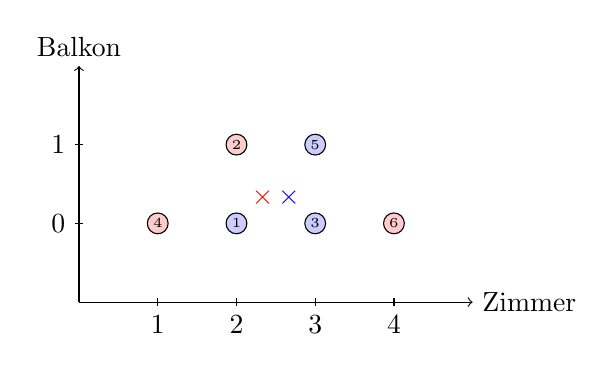
\begin{tikzpicture}
				\draw[->] (0,0) -- (5,0) node[right] {Zimmer};
				\draw[->] (0,0) -- (0,3) node[above] {Balkon};
				
				\draw (0.05,1) -- (-0.05,1) node[left] {0};
				\draw (0.05,2) -- (-0.05,2) node[left] {1};
				\draw (1,0.05) -- (1,-0.05) node[below] {1};
				\draw (2,0.05) -- (2,-0.05) node[below] {2};
				\draw (3,0.05) -- (3,-0.05) node[below] {3};
				\draw (4,0.05) -- (4,-0.05) node[below] {4};
				
				\node[circle,draw=black, fill=red!20,inner sep=1pt,outer sep=0pt] at (1,1) {\tiny 4};
				\node[circle,draw=black, fill=blue!20,inner sep=1pt,outer sep=0pt] at (2,1) {\tiny 1};
				\node[circle,draw=black, fill=blue!20,inner sep=1pt,outer sep=0pt] at (3,1) {\tiny 3};
				\node[circle,draw=black, fill=red!20,inner sep=1pt,outer sep=0pt] at (4,1) {\tiny 6};
				\node[circle,draw=black, fill=red!20,inner sep=1pt,outer sep=0pt] at (2,2) {\tiny 2};
				\node[circle,draw=black, fill=blue!20,inner sep=1pt,outer sep=0pt] at (3,2) {\tiny 5};
				
				\node[blue] at (8/3,4/3) {$\times$};
				\node[red] at (7/3,4/3) {$\times$};
			\end{tikzpicture}
			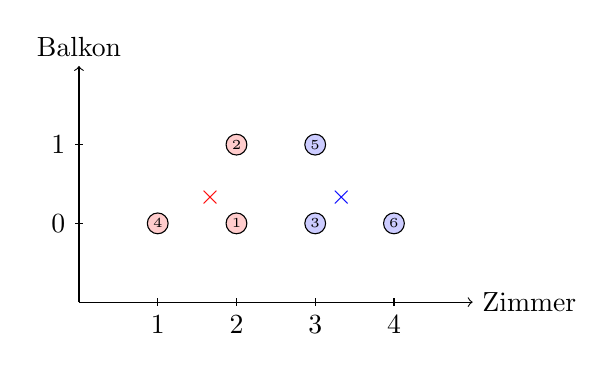
\begin{tikzpicture}
				\draw[->] (0,0) -- (5,0) node[right] {Zimmer};
				\draw[->] (0,0) -- (0,3) node[above] {Balkon};
				
				\draw (0.05,1) -- (-0.05,1) node[left] {0};
				\draw (0.05,2) -- (-0.05,2) node[left] {1};
				\draw (1,0.05) -- (1,-0.05) node[below] {1};
				\draw (2,0.05) -- (2,-0.05) node[below] {2};
				\draw (3,0.05) -- (3,-0.05) node[below] {3};
				\draw (4,0.05) -- (4,-0.05) node[below] {4};
				
				\node[circle,draw=black, fill=red!20,inner sep=1pt,outer sep=0pt] at (1,1) {\tiny 4};
				\node[circle,draw=black, fill=red!20,inner sep=1pt,outer sep=0pt] at (2,1) {\tiny 1};
				\node[circle,draw=black, fill=blue!20,inner sep=1pt,outer sep=0pt] at (3,1) {\tiny 3};
				\node[circle,draw=black, fill=blue!20,inner sep=1pt,outer sep=0pt] at (4,1) {\tiny 6};
				\node[circle,draw=black, fill=red!20,inner sep=1pt,outer sep=0pt] at (2,2) {\tiny 2};
				\node[circle,draw=black, fill=blue!20,inner sep=1pt,outer sep=0pt] at (3,2) {\tiny 5};
				
				\node[blue] at (10/3,4/3) {$\times$};
				\node[red] at (5/3,4/3) {$\times$};
			\end{tikzpicture}
		\end{center}
		\item Ablauf des Algorithmus: $C_1$ und $C_2$ stehen für die \textcolor{blue}{Cluster 1} und \textcolor{red}{2}, $\bar{C}_1$ und $\bar{C}_2$ für die Mittelwerte der Cluster 1 und 2
		\begin{center}
			\begin{tabular}{c|c|c|c|c}
				Iteration & $C_1$ & $C_2$ & $\bar{C}_1$ & $\bar{C}_2$ \\
				\hline
				0 & 1,3,4,6 & 2,5 & $\left(\frac{5}{2},0\right)$ & $\left(\frac{5}{2},1\right)$
			\end{tabular}
		\end{center}
		\begin{center}
			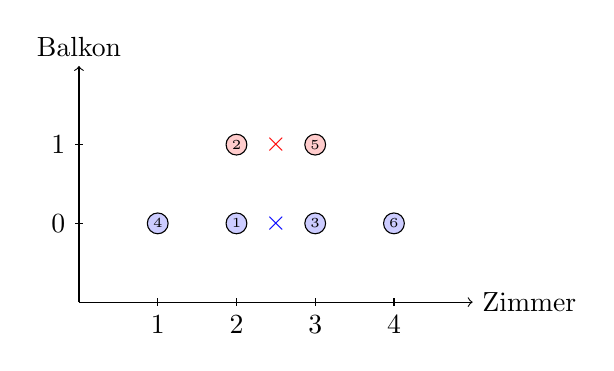
\begin{tikzpicture}
				\draw[->] (0,0) -- (5,0) node[right] {Zimmer};
				\draw[->] (0,0) -- (0,3) node[above] {Balkon};
				
				\draw (0.05,1) -- (-0.05,1) node[left] {0};
				\draw (0.05,2) -- (-0.05,2) node[left] {1};
				\draw (1,0.05) -- (1,-0.05) node[below] {1};
				\draw (2,0.05) -- (2,-0.05) node[below] {2};
				\draw (3,0.05) -- (3,-0.05) node[below] {3};
				\draw (4,0.05) -- (4,-0.05) node[below] {4};
				
				\node[circle,draw=black, fill=blue!20,inner sep=1pt,outer sep=0pt] at (1,1) {\tiny 4};
				\node[circle,draw=black, fill=blue!20,inner sep=1pt,outer sep=0pt] at (2,1) {\tiny 1};
				\node[circle,draw=black, fill=blue!20,inner sep=1pt,outer sep=0pt] at (3,1) {\tiny 3};
				\node[circle,draw=black, fill=blue!20,inner sep=1pt,outer sep=0pt] at (4,1) {\tiny 6};
				\node[circle,draw=black, fill=red!20,inner sep=1pt,outer sep=0pt] at (2,2) {\tiny 2};
				\node[circle,draw=black, fill=red!20,inner sep=1pt,outer sep=0pt] at (3,2) {\tiny 5};
				
				\node[blue] at (2.5,1) {$\times$};
				\node[red] at (2.5,2) {$\times$};
			\end{tikzpicture}
		\end{center}
		\item Ablauf des Algorithmus: $C_1$ und $C_2$ stehen für die \textcolor{blue}{Cluster 1} und \textcolor{red}{2}, $\bar{C}_1$ und $\bar{C}_2$ für die Mittelwerte der Cluster 1 und 2
		\begin{center}
			\begin{tabular}{c|c|c|c|c}
				Iteration & $C_1$ & $C_2$ & $\bar{C}_1$ & $\bar{C}_2$ \\
				\hline
				0 & 1,3,4 & 2,5,6 & $\left(2,0\right)$ & $\left(3,\frac{2}{3}\right)$ \\
				1 & 1,2,4 & 3,5,6 & $\left(\frac{5}{3},\frac{1}{3}\right)$ & $\left(\frac{10}{3},\frac{1}{3}\right)$
			\end{tabular}
		\end{center}
		\begin{center}
			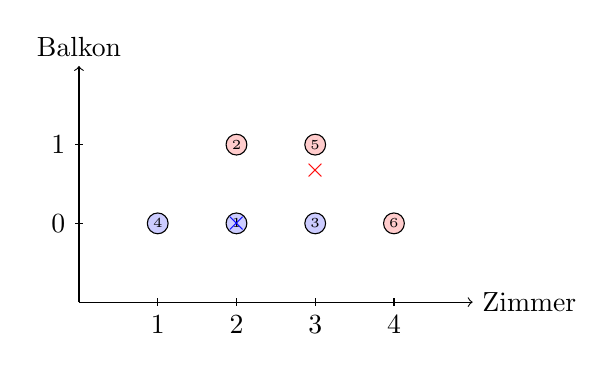
\begin{tikzpicture}
				\draw[->] (0,0) -- (5,0) node[right] {Zimmer};
				\draw[->] (0,0) -- (0,3) node[above] {Balkon};
				
				\draw (0.05,1) -- (-0.05,1) node[left] {0};
				\draw (0.05,2) -- (-0.05,2) node[left] {1};
				\draw (1,0.05) -- (1,-0.05) node[below] {1};
				\draw (2,0.05) -- (2,-0.05) node[below] {2};
				\draw (3,0.05) -- (3,-0.05) node[below] {3};
				\draw (4,0.05) -- (4,-0.05) node[below] {4};
				
				\node[circle,draw=black, fill=blue!20,inner sep=1pt,outer sep=0pt] at (1,1) {\tiny 4};
				\node[circle,draw=black, fill=blue!20,inner sep=1pt,outer sep=0pt] at (2,1) {\tiny 1};
				\node[circle,draw=black, fill=blue!20,inner sep=1pt,outer sep=0pt] at (3,1) {\tiny 3};
				\node[circle,draw=black, fill=red!20,inner sep=1pt,outer sep=0pt] at (4,1) {\tiny 6};
				\node[circle,draw=black, fill=red!20,inner sep=1pt,outer sep=0pt] at (2,2) {\tiny 2};
				\node[circle,draw=black, fill=red!20,inner sep=1pt,outer sep=0pt] at (3,2) {\tiny 5};
				
				\node[blue] at (2,1) {$\times$};
				\node[red] at (3,5/3) {$\times$};
			\end{tikzpicture}
			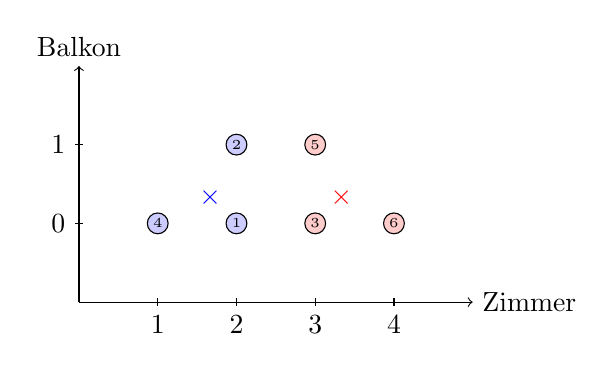
\begin{tikzpicture}
				\draw[->] (0,0) -- (5,0) node[right] {Zimmer};
				\draw[->] (0,0) -- (0,3) node[above] {Balkon};
				
				\draw (0.05,1) -- (-0.05,1) node[left] {0};
				\draw (0.05,2) -- (-0.05,2) node[left] {1};
				\draw (1,0.05) -- (1,-0.05) node[below] {1};
				\draw (2,0.05) -- (2,-0.05) node[below] {2};
				\draw (3,0.05) -- (3,-0.05) node[below] {3};
				\draw (4,0.05) -- (4,-0.05) node[below] {4};
				
				\node[circle,draw=black, fill=blue!20,inner sep=1pt,outer sep=0pt] at (1,1) {\tiny 4};
				\node[circle,draw=black, fill=blue!20,inner sep=1pt,outer sep=0pt] at (2,1) {\tiny 1};
				\node[circle,draw=black, fill=red!20,inner sep=1pt,outer sep=0pt] at (3,1) {\tiny 3};
				\node[circle,draw=black, fill=red!20,inner sep=1pt,outer sep=0pt] at (4,1) {\tiny 6};
				\node[circle,draw=black, fill=blue!20,inner sep=1pt,outer sep=0pt] at (2,2) {\tiny 2};
				\node[circle,draw=black, fill=red!20,inner sep=1pt,outer sep=0pt] at (3,2) {\tiny 5};
				
				\node[blue] at (5/3,4/3) {$\times$};
				\node[red] at (10/3,4/3) {$\times$};
			\end{tikzpicture}
		\end{center}
		\item Ablauf des Algorithmus: $C_1$ und $C_2$ stehen für die \textcolor{blue}{Cluster 1} und \textcolor{red}{2}, $\bar{C}_1$ und $\bar{C}_2$ für die Mittelwerte der Cluster 1 und 2
		\begin{center}
			\begin{tabular}{c|c|c|c|c}
				Iteration & $C_1$ & $C_2$ & $\bar{C}_1$ & $\bar{C}_2$ \\
				\hline
				0 & 1,4 & 2,3,5,6 & $\left(\frac{3}{2},0\right)$ & $\left(3,\frac{1}{2}\right)$
			\end{tabular}
		\end{center}
		\begin{center}
			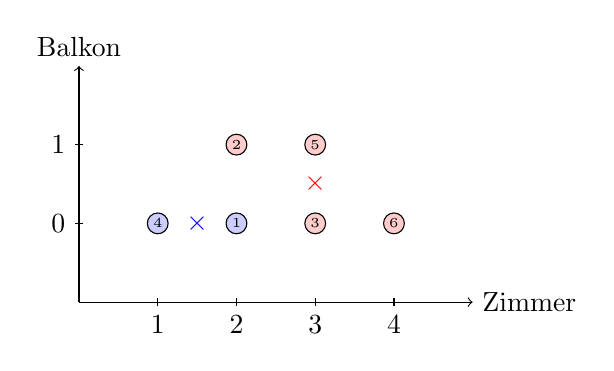
\begin{tikzpicture}
			\draw[->] (0,0) -- (5,0) node[right] {Zimmer};
			\draw[->] (0,0) -- (0,3) node[above] {Balkon};
			
			\draw (0.05,1) -- (-0.05,1) node[left] {0};
			\draw (0.05,2) -- (-0.05,2) node[left] {1};
			\draw (1,0.05) -- (1,-0.05) node[below] {1};
			\draw (2,0.05) -- (2,-0.05) node[below] {2};
			\draw (3,0.05) -- (3,-0.05) node[below] {3};
			\draw (4,0.05) -- (4,-0.05) node[below] {4};
			
			\node[circle,draw=black, fill=blue!20,inner sep=1pt,outer sep=0pt] at (1,1) {\tiny 4};
			\node[circle,draw=black, fill=blue!20,inner sep=1pt,outer sep=0pt] at (2,1) {\tiny 1};
			\node[circle,draw=black, fill=red!20,inner sep=1pt,outer sep=0pt] at (3,1) {\tiny 3};
			\node[circle,draw=black, fill=red!20,inner sep=1pt,outer sep=0pt] at (4,1) {\tiny 6};
			\node[circle,draw=black, fill=red!20,inner sep=1pt,outer sep=0pt] at (2,2) {\tiny 2};
			\node[circle,draw=black, fill=red!20,inner sep=1pt,outer sep=0pt] at (3,2) {\tiny 5};
			
			\node[blue] at (1.5,1) {$\times$};
			\node[red] at (3,1.5) {$\times$};
			\end{tikzpicture}
		\end{center}
	\end{enumerate}

	\section*{Aufgabe 3}
	Als allererstes Verändern wir unsere Datenmatrix, dass sie den Anforderungen der Aufgabenstellung entspricht:
	\begin{center}
		\begin{tabular}{c|ccccc}
			& \multicolumn{5}{c}{Merkmale} \\
			\cline{2-6}
			Wohnung & $x_1$ & $x_2$ & $x_3$ & $x_4$ & $x_5$ \\
			\hline
			1 & 1 & 1 & 0 & 0 & 0 \\
			2 & 1 & 1 & 0 & 0 & 1 \\
			3 & 1 & 1 & 1 & 0 & 0 \\
			4 & 1 & 0 & 0 & 0 & 0 \\
			5 & 1 & 1 & 1 & 0 & 1 \\
			6 & 1 & 1 & 1 & 1 & 0
		\end{tabular}
	\end{center}
	\begin{enumerate}[label=(\alph*)]
		\item Wir starten im ersten Schritt mit 6 Clustern und berechnen zu jedem die Ähnlichkeit
		\begin{center}
			\begin{tabular}{c|cccccc}
				& $\{1\}$ & $\{2\}$ & $\{3\}$ & $\{4\}$ & $\{5\}$ & $\{6\}$ \\
				\hline
				$\{1\}$ & 1 & $\frac{4}{5}$ & $\frac{4}{5}$ & $\frac{4}{5}$ & $\frac{3}{5}$ & $\frac{3}{5}$ \\
				$\{2\}$ & & 1 & $\frac{3}{5}$ & $\frac{3}{5}$ & $\frac{4}{5}$ & $\frac{2}{5}$ \\
				$\{3\}$ & & & 1 & $\frac{3}{5}$ & $\frac{4}{5}$ & $\frac{4}{5}$ \\
				$\{4\}$ & & & & 1 & $\frac{2}{5}$ & $\frac{2}{5}$ \\
				$\{5\}$ & & & & & 1 & $\frac{3}{5}$ \\
				$\{6\}$ & & & & & & 1
			\end{tabular}
		\end{center}
		Jetzt bilden wir neue Cluster:
		\begin{center}
			\begin{tabular}{c|ccc}
				& $\{1,2\}$ & $\{3,5\}$ & $\{4,6\}$ \\
				\hline
				$\{1,2\}$ & 1 & $\frac{3}{5}$ & $\frac{2}{5}$ \\
				$\{3,5\}$ & & 1 & $\frac{2}{5}$ \\
				$\{4,6\}$ & & & 1
			\end{tabular}
		\end{center}
		Und nun werden noch einmal neue Cluster gebildet:
		\begin{center}
			\begin{tabular}{c|cc}
				& $\{1,2,3,5\}$ & $\{4,6\}$ \\
				\hline
				$\{1,2,3,5\}$ & 1 & $\frac{2}{5}$ \\
				$\{4,6\}$ & & 1
			\end{tabular}
		\end{center}
		Im letzten Schritt vereinigen wir nun auch noch diese beiden Cluster und erhalten $\{1,2,3,4,5,6\}$. Das Dendrogramm ist
		\begin{center}
			\begin{tikzpicture}
			\draw[->] (0,0) -- (7,0);
			\draw[->] (0,0) -- (0,5) node[above] {Distanz $= 1-s$};
			
			\draw (1,0.05) -- (1,-0.05) node[below] {1};
			\draw (2,0.05) -- (2,-0.05) node[below] {2};
			\draw (3,0.05) -- (3,-0.05) node[below] {3};
			\draw (4,0.05) -- (4,-0.05) node[below] {5};
			\draw (5,0.05) -- (5,-0.05) node[below] {4};
			\draw (6,0.05) -- (6,-0.05) node[below] {6};
			
			\draw (0.05,1) -- (-0.05,1) node[left] {$\frac{1}{5}$};
			\draw (0.05,2) -- (-0.05,2) node[left] {$\frac{2}{5}$};
			\draw (0.05,3) -- (-0.05,3) node[left] {$\frac{3}{5}$};
			\draw (0.05,4) -- (-0.05,4) node[left] {$\frac{4}{5}$};
			
			\draw (1,0) -- (1,1) -- (2,1) -- (2,0);
			\draw (3,0) -- (3,1) -- (4,1) -- (4,0);
			\draw (5,0) -- (5,3) -- (6,3) -- (6,0);
			\draw (1.5,1) -- (1.5,2) -- (3.5,2) -- (3.5,1);
			\draw (2.5,2) -- (2.5,3) -- (5.5,3);
			\end{tikzpicture}
		\end{center}
		\item Der erste Schritt ist hier identisch, für den zweiten Schritt ergibt sich
		\begin{center}
			\begin{tabular}{c|ccc}
				& $\{1,2\}$ & $\{3,5\}$ & $\{4,6\}$ \\
				\hline
				$\{1,2\}$ & 1 & $\frac{4}{5}$ & $\frac{4}{5}$ \\
				$\{3,5\}$ & & 1 & $\frac{4}{5}$ \\
				$\{4,6\}$ & & & 1
			\end{tabular}
		\end{center}
		Und nun werden noch einmal neue Cluster gebildet:
		\begin{center}
			\begin{tabular}{c|cc}
				& $\{1,2,3,5\}$ & $\{4,6\}$ \\
				\hline
				$\{1,2,3,5\}$ & 1 & $\frac{4}{5}$ \\
				$\{4,6\}$ & & 1
			\end{tabular}
		\end{center}
		Im letzten Schritt vereinigen wir nun auch noch diese beiden Cluster und erhalten $\{1,2,3,4,5,6\}$. Das Dendrogramm ist
		\begin{center}
			\begin{tikzpicture}
			\draw[->] (0,0) -- (7,0);
			\draw[->] (0,0) -- (0,5) node[above] {Distanz $= 1-s$};
			
			\draw (1,0.05) -- (1,-0.05) node[below] {1};
			\draw (2,0.05) -- (2,-0.05) node[below] {2};
			\draw (3,0.05) -- (3,-0.05) node[below] {3};
			\draw (4,0.05) -- (4,-0.05) node[below] {5};
			\draw (5,0.05) -- (5,-0.05) node[below] {4};
			\draw (6,0.05) -- (6,-0.05) node[below] {6};
			
			\draw (0.05,1) -- (-0.05,1) node[left] {$\frac{1}{5}$};
			\draw (0.05,2) -- (-0.05,2) node[left] {$\frac{2}{5}$};
			\draw (0.05,3) -- (-0.05,3) node[left] {$\frac{3}{5}$};
			\draw (0.05,4) -- (-0.05,4) node[left] {$\frac{4}{5}$};
			
			\draw (1,0) -- (1,1) -- (2,1) -- (2,0);
			\draw (3,0) -- (3,1) -- (4,1) -- (4,0);
			\draw (5,0) -- (5,3) -- (6,3) -- (6,0);
			\draw (1.5,1) -- (3.5,1);
			\draw (2.5,1) -- (4.5,1) -- (4.5,3) -- (5.5,3);
			\end{tikzpicture}
		\end{center}
	\end{enumerate}
\end{document}